\documentclass[10pt]{article}
\usepackage{../../local}
\usepackage{booktabs}
\usepackage{framed}
\usepackage{mathrsfs}

\newcommand{\classcode}{Physics 137B}
\newcommand{\classname}{Quantum Mechanics II}
\renewcommand{\maketitle}{%
\hrule height4pt
\large{Eric Du \hfill \classcode}
\newline
\large{HW 05} \Large{\hfill \classname \hfill} \large{\today}
\hrule height4pt \vskip .7em
\normalsize
}
\linespread{1.1}
\begin{document}
		\maketitle
		\section*{Collaborators}
		I worked with \textbf{Andrew Binder} to complete this assignment. Sorry for the late submission, most of the time spent doing this problem set was actually typing up the solutions rather than doing the problems themselves.

		\section*{Problem 1}
		Derive the fine structure formula (Equation 7.68) from the relatistic correction (Equation 
		7.58) and the spin-orbit coupling (Equation 7.67). \textit{Hint:} Note that $j = \ell \pm 1/2$
		(except for $\ell = 0$, where only the plus sign occurs); treat the plus sign and the minus 
		sign separately, and you'll find that you get the same final answer either way.

		\begin{solution}
			We use $j = l \pm \frac 12$, following the hint. Starting with
			$J = l + \frac 12$, recall the spin-orbit corrections written
			in terms of $l$:

			\[ E_{\text{rel}} = -\frac{E_n^2}{2mc^2} 
			\left[\frac{4n}{n+ 1/2} - 3\right] \phantom{aaaa} E_{\text{SO}} = \frac{E_n^2}{mc^2}\left[\frac{n\left(j(j+1) 
			- l(l+1)-\frac34\right)}{l\left(l+1/2\right)(l+1)}\right]\]

			Now using the relation that $l = j - 1/2$, we can get the 
			following corrections:
			
			\begin{align*}
				E_{\text{rel}} &= -\frac{E_n^2}{2mc^2} \left[ \frac{4n}{j} - 3\right]\\
				E_{\text{SO}} &= \frac{E_n^2}{mc^2}\left[ \frac{n(j(j+1) - (j - 1/2)(j + 1/2) - 3/4)}{(j - 1/2)j(j+1/2)}\right]\\
				&= \frac{E_n^2}{mc^2}\left[\frac{n(j - 1/2)}{(j - 1/2)j(j+1/2)}\right]\\
				&= \frac{E_n^2 n}{mc^2j(j + 1/2)}
			\end{align*}

			Adding these together to get the fine structure correction:
			\begin{align*}
				E_{\text{FS}} &= \frac{E_n^2}{mc^2}\left( \frac{n}{j(j + 1/2)}\right) - \frac{E_n^2}{2mc^2}\left( \frac{4n}{j} - 3\right)\\
				&= \frac{E_n^2}{mc}\left( \frac{n}{j(j + 1/2)} - 1/2\left( \frac{4n}{j} - 3\right) \right)\\
				&= \frac{E_n^2}{mc} \left( \frac{n}{j(j+1/2)} - \frac{2n}{j} + \frac 32\right) \\
				&= \frac{E_n^2}{2mc}\left[ \frac{2(n - 2n(j + 1/2))}{j + 1/2} + 3\right]\\
				&= \frac{E_n^2}{2mc}\left[ 3 - \frac{4nj}{j(j + 1/2)}\right]\\
				&= \frac{E_n^2}{2mc}\left[ 3 - \frac{4n}{j + 1/2}\right]
			\end{align*}

			Which is the fine structure, as desired. Now using $j = l - 1/2$, we get the following corrections for the relativistic and 
			spin orbit corrections:

			\begin{align*}
				E_{\text{rel}} &= -\frac{E_n^2}{2mc^2}\left(\frac{4n}{j + 1} - 3\right)\\
				E_{\text{SO}} &= \frac{E_n^2}{mc^2}\left(-\frac{n}{(j + 1/2)(j+1)}\right)
			\end{align*}

			Adding the two together, we get:

			\begin{align*}
				E_{\text{FS}} &= -\frac{E_n^2}{2mc^2}\left(\frac{4n}{j + 1} - 3\right) + \frac{E_n^2}{mc^2}\left(-\frac{n}{(j + 1/2)(j+1)}\right)\\
				&= -\frac{E_n^2}{2mc^2}\left[ \frac{4n}{j+1} - 3 + \frac{2n}{(j + 1/2)(j + 1)}\right]\\
				&= -\frac{E_n^2}{2mc^2}\left[ \frac{4n(j + 1/2) + 2n}{(j+1)(j + 1/2)} - 3\right]\\
				&= -\frac{E_n^2}{2mc^2}\left[\frac{4n(j + 1)}{(j+1)(j+1/2)} - 3\right]\\
				&= \frac{E_n^2}{2mc^2}\left[ 3 - \frac{4n}{j + 1/2}\right]
			\end{align*}
			as desired. 
		\end{solution}

		\pagebreak

		\section*{Problem 2}
		The most prominent feature of the hydrogen spectrum in the visible region is the Balmer line,
		coming from the transition $n=3$ to $n=2$. First of all, determine the wavelength and frequency
		of this line according to the Bohr theory .Fine structure splits this line into several closely
		spaced lines; the question is: \textit{How many, and what is their spacing? Hint:} First 
		determine how many sublevels the $n=2$ level splits into, and find $E_{fs}^1$ for each of 
		these, in eV. Then do the same for $n=3$. Draw an energy level diagram showing all possible
		transitions from $n=3$ to $n=2$. The energy released (in the form of a photon) is 
		$(E_3 - E_2) + \Delta E$, the first part being common to all of them, and $\Delta E$ (due to 
		fine structure) varying from one transition to the next. Find $\Delta E$ (in eV) for each 
		transition. Finally, convert to photon frequency, and determine the spacing between adjacent
		spectral lines (in Hz) -- \textit{not} the frequency interval between each line and the 
		\textit{unperturbed} line, (which is, of course, unobservable), but the frequency interval 
		between each line and the \textit{next} one. Your final answer should take the form: ``The red
		Balmer line splits into (???) lines. In order of increasing frequency, they come from the 
		transitions (1) $j = (???)$ to $j = (???)$, (2) $j = (???)$ to $j = (???), \dots$. The 
		frequency spacing between line (1) and line (2) is (???) Hz, the spacing between line (2) and 
		line (3) is (???) Hz, $\dots$.''

		\begin{solution}
			The energy transition is from $n = 3$ to $n = 2$, so the change in energy is given by: 
			\[ \Delta E = E_3 - E_2 = E_1 \left( \frac 19 - \frac 14\right) = -\frac{5E_1^0}{36}\]
			Solving for the wavelength, we get: 
			\[ \frac{2\pi \hbar c}{\lambda} = -\frac{5E_1^0}{36} \implies \lambda \approx 655 \text{ nm}\]
			And we can also solve for $f$: 
			\[ f = \frac{c}{\lambda} \approx 4.58 \times 10^{14} \text{ Hz}\]
			Now we are asked to determine how the fine structure splits these two lines. We will follow the hint closely to arrive at the final answer. First, based on the fine-structure correction, we know that (from the previous problem)
			\[ E_{FS} = \frac{E_n^2}{2mc^2}\left[ 3 - \frac{4n}{(j + 1/2)}\right]\]
			So the degeneracy lies in $j = l + 1/2$. For $n = 2$, we have $l = 0$ or $l = 1$, so the fine structure splits this into two energy levels (recall that $j = l + 1/2$): 
			\begin{align*}
				l &= 0 \ (j = 1/2): \ \ \ E_2^1 = \frac{E_2^2}{2mc^2}\left( 3 - \frac{4(2)}{1/2 + 1/2}\right) = -\frac{5E_2^2}{2mc^2} = -\frac{5}{32} \frac{E_1^2}{mc^2} \approx -5.66 \times 10^{-5} \text{ eV}\\
				l &= 1 \ (j = 3/2): \ \ \ E_2^1 = \frac{E_2^2}{2mc^2} \left( 3 - \frac{4(2)}{(3/2 + 1/2)}\right) = -\frac{E_2^2}{2mc^2} = -\frac{1}{32} \frac{E_1^2}{mc^2} \approx -1.13 \times 10^{-5} \text{ eV}
			\end{align*}
			For the $n=3$ case, we now have $l = 0, 1, 2$ so the fine structure will split this into three energy levels:
			\begin{align*}
				l &= 0 \ (j = 1/2): \ \ \ E_3^1 = \frac{E_3^2}{2mc^2}\left( 3 - \frac{4(3)}{1/2 + 1/2}\right) = -\frac{9E_3^2}{2mc^2} = -\frac{1}{18} \frac{E_1^2}{mc^2} \approx 2.01 \times 10^{-5} \text{ eV}\\
				l &= 1 \ (j = 3/2): \ \ \ E_3^1 = \frac{E_3^2}{2mc^2}\left( 3 - \frac{4(3)}{3/2 + 1/2}\right) = -\frac{3E_3^2}{2mc^2} = -\frac{1}{54} \frac{E_1^2}{mc^2} \approx -0.67 \times 10^{-5} \text{ eV}\\
				l &= 2 \ (j = 5/2): \ \ \ E_3^1 = \frac{E_3^2}{2mc^2}\left( 3 - \frac{4(3)}{5/2 + 1/2}\right) = -\frac{E_3^2}{2mc^2} = -\frac{1}{162} \frac{E_1^2}{mc^2} \approx -0.22 \times 10^{-5} \text{ eV}
			\end{align*}

			We can plot these to see what the transitions look like (credit goes to Andrew Binder for the Ti\textit{k}Z diagram):

			\begin{center}
				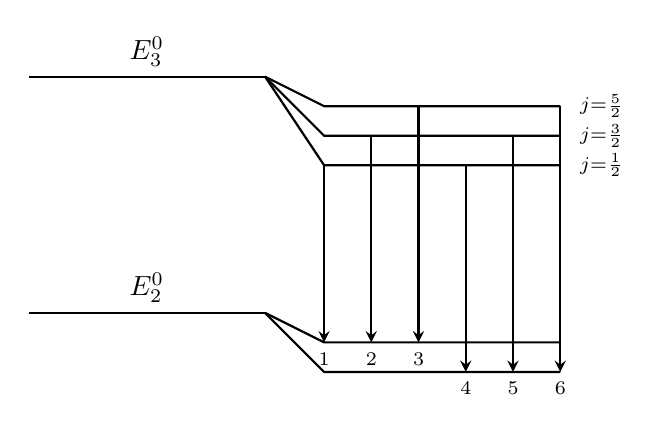
\begin{tikzpicture}[scale=1.5]
					\draw[thick, -] (0,2) -- (2,2) node[midway,above] {$E_2^0$} (0,4) -- (2,4) node[midway,above] {$E_3^0$};
					\foreach \x in {0.25,0.5} {
						\draw[thick] (2,2) -- (2.5,2-\x) -- (4.5,2-\x);
					}
					\foreach \x in {0.25,0.5,0.75} {
						\draw[thick] (2,4) -- (2.5,4-\x) -- (4.5,4-\x);
					}
					\node at (4.85,3.75) (1) {$\scriptstyle j = \frac{5}{2}$};
					\node at (4.85,3.5)  (2) {$\scriptstyle j = \frac{3}{2}$};
					\node at (4.85,3.25) (3) {$\scriptstyle j = \frac{1}{2}$};
					\draw[thick, -stealth] (2.5,3.25) -- (2.5,1.75) node[anchor=north] {$\scriptstyle1$};
					\draw[thick, -stealth] (2.9,3.5)  -- (2.9,1.75) node[anchor=north] {$\scriptstyle2$};
					\draw[thick, -stealth] (3.3,3.75) -- (3.3,1.75) node[anchor=north] {$\scriptstyle3$};
					\draw[thick, -stealth] (3.7,3.25) -- (3.7,1.5)  node[anchor=north] {$\scriptstyle4$};
					\draw[thick, -stealth] (4.1,3.5)  -- (4.1,1.5)  node[anchor=north] {$\scriptstyle5$};
					\draw[thick, -stealth] (4.5,3.75) -- (4.5,1.5)  node[anchor=north] {$\scriptstyle6$};
				\end{tikzpicture}
			\end{center}
			So we have six transitions to calculate the energy for. In terms of the notation, I will label $E_{k, m}$ to denote the change in energy from the $k$-th state in $n=3$ to the $m$-th state in $n=2$ with the states arranged in order of increasing $j$. So for instance, $E_{1, 2}$ would correspond to the transition from the lowest energy state in $E_3$ in the split down to the highest eneryg state in $E_2$.
			\begin{align*}
				\Delta E_{1, 2} &= \left(-\frac{1}{18} + \frac{1}{32}\right) \frac{E_1^2}{mc^2} \approx 8.8 \times 10^{-6} \text{ eV}\\
				\Delta E_{2, 2} &= \left(-\frac{1}{54} + \frac{1}{32}\right) \frac{E_1^2}{mc^2} \approx 4.6 \times 10^{-6} \text{ eV}\\
				\Delta E_{3, 2} &= \left(-\frac{1}{162} + \frac{1}{32}\right) \frac{E_1^2}{mc^2} \approx 9.1 \times 10^{-6} \text{ eV}\\
				\Delta E_{1, 1} &= \left(-\frac{1}{18} + \frac{5}{32}\right) \frac{E_1^2}{mc^2} \approx 36.5 \times 10^{-6} \text{ eV} \\
				\Delta E_{2, 1} &= \left(-\frac{1}{54} + \frac{5}{32}\right) \frac{E_1^2}{mc^2} \approx 49.9 \times 10^{-6} \text{ eV}\\
				\Delta E_{3, 1} &= \left(-\frac{1}{162} + \frac{5}{32}\right) \frac{E_1^2}{mc^2} \approx 54.3 \times 10^{-6} \text{ eV}
			\end{align*}
			So now finally writing out the answer in the format from the hint: 

			The red balmer line splits into 6 lines. In order of increasing frequency, they come from the following transitions: 

			\begin{itemize}
				\item $j = 1/2$ to $j = 3/2$
				\item $j = 3/2$ to $j = 3/2$
				\item $j = 5/2$ to $j = 5/2$
				\item $j = 1/2$ to $j = 1/2$
				\item $j = 3/2$ to $j = 1/2$
				\item $j = 5/2$ to $j = 1/2$
			\end{itemize}

			The frequency spacing between line (1) and line (2) is $3.23 \times 10^{9}$ Hz, the spacing between line (2) and (3) is $1.08 \times 10^{9}$ Hz, the spacing between line (3) and (4) is $6.60 \times 10^{9}$ Hz, the spacing between line (4) and (5) is $3.23 \times 10^{9}$ Hz, and finally the spacing between line (5) and (6) is $1.08 \times 10^{9}$ Hz. In general, the frequency spacing between line $n$ and line $n+1$ is given by 

			\[ f_n = \frac{\Delta E_{n+1} - \Delta E_n}{2\pi \hbar}\]
		\end{solution}
		\pagebreak

		\section*{Problem 3}
		Consider the (eight) $n=2$ states $\ket{2\ell \ j \ m_j}$. Find the energy of each state, under
		weak-field Zeeman splitting, and construct a diagram like Figure 710 to show how the energies
		evolve as $B_{ext}$ increases. Label each line clearly, and indicate its slope. 

		\begin{solution}
			For $n=2$, we have 8 stattes, which we will label $\ket{n}$:

			\begin{align*}
				\ket{1} &= \textstyle\ket{2,0,1/2,-1/2}\\
				\ket{2} &= \textstyle\ket{2,0,1/2,1/2}\\
				\ket{3} &= \textstyle\ket{2,1,1/2,-1/2}\\
				\ket{4} &= \textstyle\ket{2,1,1/2,1/2}\\
				\ket{5} &= \textstyle\ket{2,1,3/2,-3/2}\\
				\ket{6} &= \textstyle\ket{2,1,3/2,-1/2}\\
				\ket{7} &= \textstyle\ket{2,1,3/2,1/2}\\
				\ket{8} &= \textstyle\ket{2,1,3/2,3/2}
			\end{align*}

			For the weak Zeeman effect, we need to consider both the fine structure energy and the Zeeman correction. Starting with the Zeeman correction, we calculate the g-factor for the states $l = 0$ with $j = 1/2$ and $l = 1$ with $j = 1/2, 3/2$: 
			\begin{align*}
				g_J^{0, 1/2} &= 1 + \frac{(1/2)(1/2 + 1) - 0(1) + 1/2(1/2 +1)}{2(1/2)(1/2 + 1)} = 1+1 = 2\\
				g_J^{1, 1/2} &= 1 + \frac{(1/2)(1/2 + 1) - 1(2) + 1/2(1/2 + 1)}{2(1/2)(3/2 + 1)} = 1 - \frac{1}{3} = \frac 23\\
				g_J^{1, 3/2} &= 1 + \frac{3/2(3/2 + 1) - 1(2) + 1/2(1/2 + 1)}{2(3/2)(3/2 + 1)} = 1 + \frac{5}{15} = \frac 43
			\end{align*}
			Now we can calculate the Zeeman effect $E_z = \mu_B g_J B_{ext}m_j$:

			\begin{align*}
				E^1_{Z, 1} &= -2\mu_B B_{ext}\\
				E^1_{Z, 2} &= 2\mu_B B_{ext}\\
				E^1_{Z, 3} &= -\frac 13\mu_B B_{ext}\\
				E^1_{Z, 4} &= \frac 13\mu_B B_{ext}\\
				E^1_{Z, 5} &= -\frac 23 \mu_B B_{ext}\\
				E^1_{Z, 6} &= \frac 23 \mu_B B_{ext}\\
				E^1_{Z, 7} &= -2\mu_B B_{ext}\\
				E^1_{Z, 8} &= 2\mu_B B_{ext}
			\end{align*}

			Now incorporating the fine structure energy, which only depends on $j$:
			\begin{align*}
				E_{FS, 1/2} &= -\frac{13.6 \text{ eV}}{2^2}\left[ 1 + \frac{\alpha^2}{2}\left( \frac{2}{1/2 + 1/2} - \frac 34\right)\right] = -3.4 \text{ eV}\left(1 + \frac{5}{16} \alpha^2\right)\\
				E_{FS, 3/2} &= -\frac{13.6 \text{ eV}}{2^2}\left[ 1 + \frac{\alpha^2}{2}\left(\frac{2}{3/2 + 1/2} - \frac 34\right) \right] = -3.4 \text{ eV}\left( 1 + \frac{1}{16}\alpha^2\right)
			\end{align*}

			Putting these together, we get: 
			\begin{align*}
				E_1 &= E_{FS, 1/2} - \mu_B B_{ext}\\
				E_2 &= E_{FS, 1/2} + \mu_B B_{ext}\\
				E_3 &= E_{FS, 1/2} - \frac 13 \mu_B B_{ext}\\
				E_4 &= E_{FS, 1/2} + \frac 13 \mu_B B_{ext}\\
				E_5 &= E_{FS, 3/2} - \frac 23 \mu_B B_{ext}\\
				E_6 &= E_{FS, 3/2} + \frac 23 \mu_B B_{ext}\\
				E_7 &= E_{FS, 3/2} - 2\mu_B B_{ext}\\
				E_8 &= E_{FS, 3/2} + 2\mu_B B_{ext}
			\end{align*}
		
			Plotting these out (again thanks to Andrew for the Ti\textit{k}Z diagram):
			
			\begin{center}
				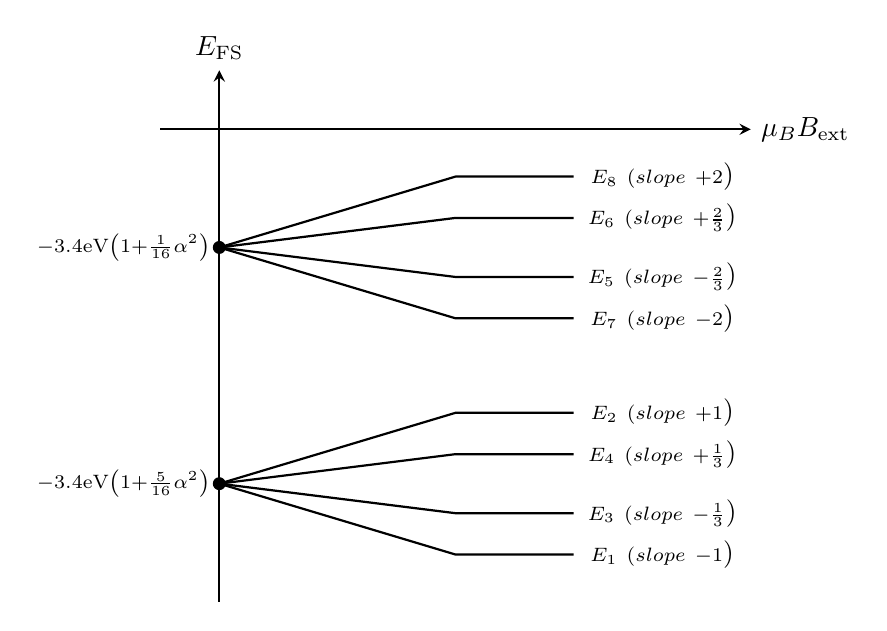
\begin{tikzpicture}[scale=1.5]
					\draw[thick, -stealth] (0,0) -- (0,4.5) node[anchor=south] {$E_{\mathrm{FS}}$};
					\draw[thick, -stealth] (-0.5,4) -- (4.5,4) node[anchor=west] {$\mu_BB_{\mathrm{ext}}$};
					\filldraw[black] (0,1) circle (0.05cm) node[anchor=east] {$\scriptstyle-3.4\mathrm{eV}\left(1 + \frac{5}{16}\alpha^2\right)$};
					\filldraw[black] (0,3) circle (0.05cm) node[anchor=east] {$\scriptstyle-3.4\mathrm{eV}\left(1 + \frac{1}{16}\alpha^2\right)$};
					\foreach \x in {-0.6,-0.25,0.25,0.6} {
						\draw[thick] (0,1) -- (2,1+\x) -- (3,1+\x);
						\draw[thick] (0,3) -- (2,3+\x) -- (3,3+\x);
					}
					\node at (3.75,0.4) (1) {$\scriptstyle E_1\ (\text{slope}\ -1$)};
					\node at (3.75,0.75) (2) {$\scriptstyle E_3\ (\text{slope}\ -\frac13$)};
					\node at (3.75,1.25) (3) {$\scriptstyle E_4\ (\text{slope}\ +\frac13$)};
					\node at (3.75,1.6) (4) {$\scriptstyle E_2\ (\text{slope}\ +1$)};
					\node at (3.75,2.4) (5) {$\scriptstyle E_7\ (\text{slope}\ -2$)};
					\node at (3.75,2.75) (6) {$\scriptstyle E_5\ (\text{slope}\ -\frac23$)};
					\node at (3.75,3.25) (7) {$\scriptstyle E_6\ (\text{slope}\ +\frac23$)};
					\node at (3.75,3.6) (8) {$\scriptstyle E_8\ (\text{slope}\ +2$)};
				\end{tikzpicture}
			\end{center}
		\end{solution}

		\pagebreak

		\section*{Problem 4}
		If $\ell = 0$, then $j =s, m_j = m_s$ and the ``good'' states are the same ($\ket{n \ m_s}$)
		for weak \textit{and} strong fields. Determine $E_Z^1$ (from Equation 7.74) and the fine
		structure energies (Equation 7.69), and write down the general result for the $l=0$ Zeeman
		effect -- \textit{regardless} of the strength of the field. Show that the strong-field 
		formula (Equation 7.86) reproduces this result, provided that we interpret the indeterminate 
		term in square brackets as 1. 

		\begin{solution}
			In the case where $l = 0$, then we have $j = s = 1/2$ and $m_j = m_s$ as a result. We can rewrite the Zeeman energy to reflect this: 
			\[ E_Z = \frac{eB_{ext}}{2m} (2 m_s \hbar) = 2m_s \mu_B B_{ext}\]
			The fine structure correction, which is dependent on $j$, then becomes: 
			\[ E_{nj} = -\frac{13.6 \text{ eV}}{n^2}\left[1 + \frac{\alpha^2}{n^2}\left( n + \frac 34\right) \right]\]
			So the total energy correction is the sum of these two: 
			\[ E = -\frac{13.6\text{ eV}}{n^2}\left[1 + \frac{\alpha^2}{n^2}\left(n - \frac 34\right) \right] + 2m_s \mu_B B_{ext}\]
			We now want to show that Equation 7.86 also reproduces this result provided that the term in square brackets is 1. Doing so, we obtain the equation: 
			\begin{align*}
				E_{fs}^1 &= \frac{13.6 \text{ eV}}{n^3}\alpha^2\left( \frac{3}{4n} - 1\right)\\
				&= \frac{13.6 \text{ eV}}{n^4} \alpha^2 \left( \frac 34 - n\right) \\
				&= -\frac{13.6 \text{ eV}}{n^4} \alpha^2 \left( n - \frac 34\right)
			\end{align*}
			So combining this back, we see that the energy correction becomes: 
			\begin{align*}
				E &= -\frac{13.6 \text{ eV}}{n^2} - \frac{13.6 \text{ eV}}{n^4} \alpha^2 \left( n - \frac 34\right) + 2m_s \mu_B B_{ext}\\
				&=-\frac{13.6 \text{ eV}}{n^2}\left[1 + \frac{\alpha^2}{n^2}\left( n - \frac 34\right) \right] + 2m_S \mu_B B_{ext}
			\end{align*}
			which is the same result as before, as desired.
		\end{solution}

		\pagebreak

		\section*{Problem 5}
		The eigenstates of a rotating dumbbell, with moment of inertia $I$\[
		E_l = \frac{\hbar^2 l(l+1)}{2I}
		\] are $(2l + 1)$-fold degenerate. In the event that the dumbbell is equally and oppositely
		charged at its ends, it becomes a dipole. The interaction energy between such a dipole and 
		a constant, uniform electric field $\mathscr E$ is \[
				\hat{H'} = -d \cdot \mathscr E \ \ (\hat{H} - \mathbf d \cdot \mathscr E)
		\] The dipole moment of the dumbbell is $\mathbf d$. Show that to terms of first order, this
		perturbing potential \textit{does not separate} the degenerate $E_l$ eigenstates.

		\begin{solution}
				I will argue this both qualitatively and quantitatively. Qualitatively speaking, we know that 
				degeneracy arises when we have symmetry in the problem, and that introducing a perturbation 
				which depends on that symmetric parameter now breaks the symmetry. For instance, the Zeeman
				effect arises when we now introduce a term which breaks the symmetry for $m_l$, causing a split
				in the energy levels as a result. 

				Since the magnetic moment is $\mathbf d = e \mathbf r$, then we know that this value actually 
				only depends on $r$, so there is no $L_z$ component, meaning that the perturbation should not 
				depend on the value of $m_l$. Since the degeneracies in this problem arise from the degeneracies
				in $m_l$, then the fact that $d$ does not depend on $m_l$ means that we should not expect it to
				separate the $E_l$ eigenstates. 

				Quantiatively, we can calculate the energy change due to this perturbation and show that it 
				is in fact equal to zero. The eigenfunctions of the dumbbell are those of the rigid rotor, which
				are the spherical harmonics. Calculating the energy correction:
				\[
						\Delta E = \expval{-\mathcal E \cdot \mathbf d}{lm} = -\mathcal E \expval{\mathbf d}{lm} 
						= -\mathcal E \expval{er}{lm} = -\mathcal E e \expval{r}{lm}
				\]
				Since $\ket{lm}$ has no $r$ component, this expectation value is zero, as expected.
		\end{solution}

		\pagebreak
		\section*{Problem 6}
		Consider again the dipole moment described in Problem 13.14. If both ends are equally charged,
		the rotating dipole constitutes a magnetic dipole. If the dipole has angular momentum 
		$\mathbf L$, the corresponding magnetic dipole moment is \[
		\boldsymbol \mu = \frac{e}{2mc}\mathbf L
		\] where $e$ is the net charge of the dipole. The interaction energy between this magnetic
		dipole and a constant, uniform magnetic field $\mathscr B$ is \[
				\hat{H'} = -\hat{\boldsymbol \mu}\cdot \mathscr B = -\frac{e}{2mc}\mathbf{\hat{L}}
				\cdot \mathscr B \ \ (\hat{H} = \hat{H_0} - \hat{\boldsymbol \mu} \cdot \mathscr B)
		\] 
		\begin{enumerate}[label=\alph*)]
				\item If $\mathscr B$ points in the $z$ direction, show that $\hat{H'}$ separates
						the $(2l+1)$-fold degenerate $E_l$ energies of the rotating dipole.

						\begin{solution}
								To show that the degeneracy splits, we show that the energy correction is 
								nonzero. If $\mathscr B$ points in the $\hat{z}$ direction, then taking the dot
								product with $L$:
								\[
								\hat{\mathbf L} \cdot \mathscr B = \hat{L_x}\mathscr B_x + \hat{L_y}\mathscr B_y
								+ \hat{L_z} \mathscr B_z = \hat{L_z}\mathscr B_z
								\] 
								Note that the first two terms go to zero because $\mathscr B$ points only in the
								$\hat{z}$ direction. Now, calculating the expectation value:

								\begin{align*}
										\expval{-\frac{e}{2mc}\hat{L}\cdot \mathscr{B}}{lm} &= -\frac{e}{2mc}
										\expval{\hat{L_z} \mathscr B_z}{lm} \\
										&= -\frac{e\mathscr B_z}{2mc}\expval{\hat{L_z}}{lm}	\\
										&= -\frac{eB_z\hbar m_l}{2mc}
								\end{align*}

						\end{solution}
				\item Apply these results to one-electron atoms to find the splitting of the $P$ 
						states. (Neglect spin-orbit coupling.) (\textit{Note:} This phenomenon is an 
						example of the \textit{Zeeman effect} discussed previously in Problems 12.15
						et seq.)

						\begin{solution}
								We repeat the same calculation as before, but now using the wavefunctions for 
								single particle atoms, which happens to just be that of the hydrogen atom:
								\begin{align*}
										\expval{-\frac{e}{2mc}\hat{L_z}\mathscr B_z}{nlm} &= 
										-\frac{e\mathscr B_z}{2mc}\expval{\hat{L_z}}{nlm}  \\
										&= -\frac{e\mathscr B_z}{2mc}\expval{\expval{\hat{L_z}}{lm}}{nl} \\
										&= -\frac{e\mathscr B_z}{2mc}\expval{\hat{L_z}}{lm} \\
										&= -\frac{e\mathscr B_z \hbar m_l}{2mc} 
								\end{align*}
						\end{solution}
		\end{enumerate}


		

\end{document}
